\section{Промоторы прокариот и регуляторные элементы. Лактозный оперон. Аттенюация на примере 
триптофанового оперона. 
Промоторы эукариот. Энхансеры и сайленсеры. 
Альтернативный сплайсинг.}

\subsection{Промотор}

\textbf{Промотор} - последовательность нуклеотидов ДНК, узнаваемая РНК-полимеразой как стартовая площадка для начала транскрипции. 

По активности промоторы делят на:
\begin{itemize}
    \item конститутивные (постоянный уровень транскрипции);
    \item индуцибельные (транскрипция зависит от условий в клетке, например от присутствия определенных веществ или наличия теплового шока).
\end{itemize}

Активация промотора определяется присутствием набора транскрипционных факторов.

\subsection{Промоторы прокариот и регуляторные элементы}
У прокариот обычно имеется общий промотр сразу для нескольких генов (ген - последовательность ДНК с информацией о том, как строить белок). Эти несколько генов называют \textbf{опероном}, они всегда транскрибируются вместе. 

\textbf{Регуляторные элементы} - это белки, регулирующие активацию промоторов. Фактически, это белки, помогающие РНК-полимеразе связаться с конкретным опероном. Регуляторные элементы реагируют на внешние раздражители по изменениям концентрации различных веществ в клетке и запускают/гасят синтез РНК тех белков, которые сейчас нужны/не нужны для выживания.

\subsection{Лактозный оперон}
В норме бактерия кушает глюкозу (сахар), и не способна кушать лактозу (дисахарид, состоящий из двух сахаров, глюкозы и галактозы (см. рис. \ref{fig:9_lactose})). Синтезировать белки, которые позволяют кушать лактозу, в присутствии глюкозы невыгодно.

Но бывают ситуации, когда в среде вокруг бактерии нет глюкозы, но есть лактоза. Тогда активизируется \textbf{лактозный оперон} и начинает транскрибироваться группа генов, кодирующая белки, позволяющие кушать лактозу. 

\begin{figure}[H]
    \centering
    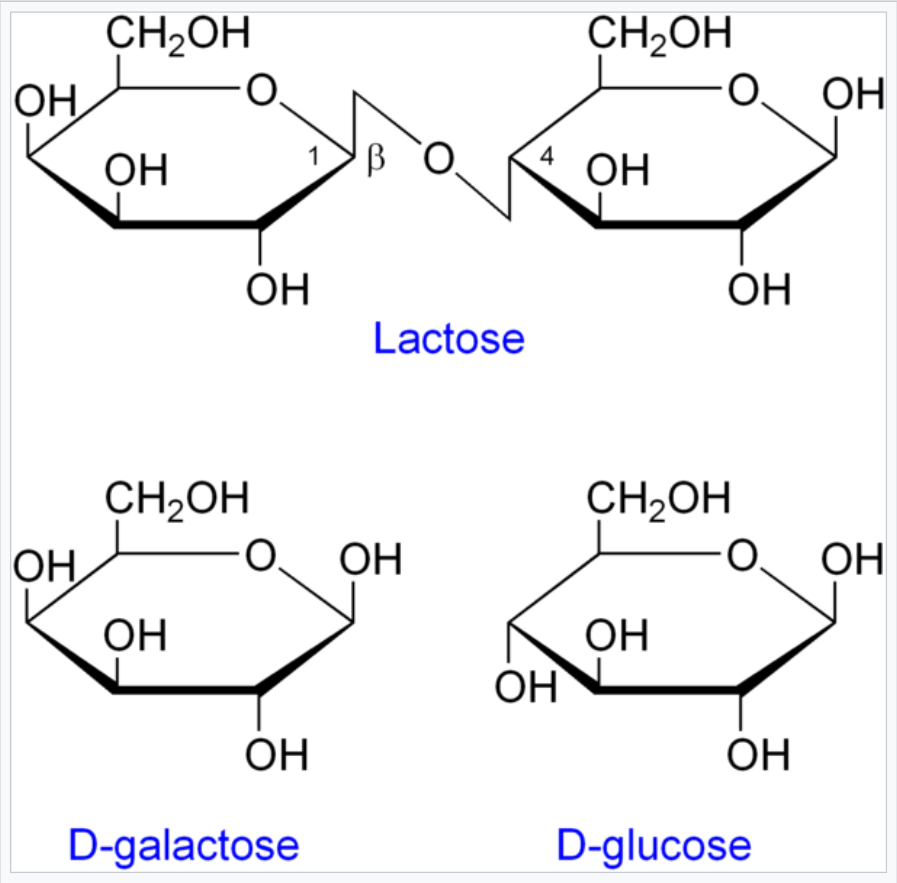
\includegraphics[width = 0.6 \linewidth]{9_lactose.png}
    \caption{Разница между глюкозой и лактозой (греческие буквы указывают конкретные изомеры феществ, то есть геометрическое строение).}
    \label{fig:9_lactose}
\end{figure}

Рассмотрим подробнее молекулярный механизм активации лактозного оперона. 

\begin{itemize}
    \item Лактозный оперон состоит из трех генов (см. рис. \ref{fig:9_glucose_on}-\ref{fig:9_lactose_on}): 
    
    a) ген lacZ, кодирует фермент \(\beta\)-галактозидазу, расщепляющий дисахарид лактозу на глюкозу и галактозу;
    
    б) ген lacY, кодирует фермент  \(\beta\)-галактозидпермеазу, протаскивающий лактозу из внешней среду в клетку через клеточную мембрану;
    
    в) третий ген, роль которого не ясна, поэтому нахуй его называть.
    
    \item Белок-репрессор в нормальных условиях сидит на операторном участке ДНК и мешает транскрипции (см. те же картинки).
    
    \item При повышенной концентрации лактозы репрессор связывается с лактозой, меняет свою форму и не может больше удерживаться на ДНК.
    
    \item Глюкоза подавляет синтез вещества цАМФ (циклическая форма аденазин-монофосфата). В отсутствии глюкозы это вещество синтезируется и дает сигнал белку CAP о клеточном голоде.
    
    \item Белок CAP садится на промотор лактозного оперона и облегчает его связывание с РНК-полимеразой.
    
    \item Запускается синтез белков, расщепляющих лактозу.
    
    
\end{itemize}

\begin{minipage}{.49\textwidth}
    \begin{figure}[H]
        \centering
        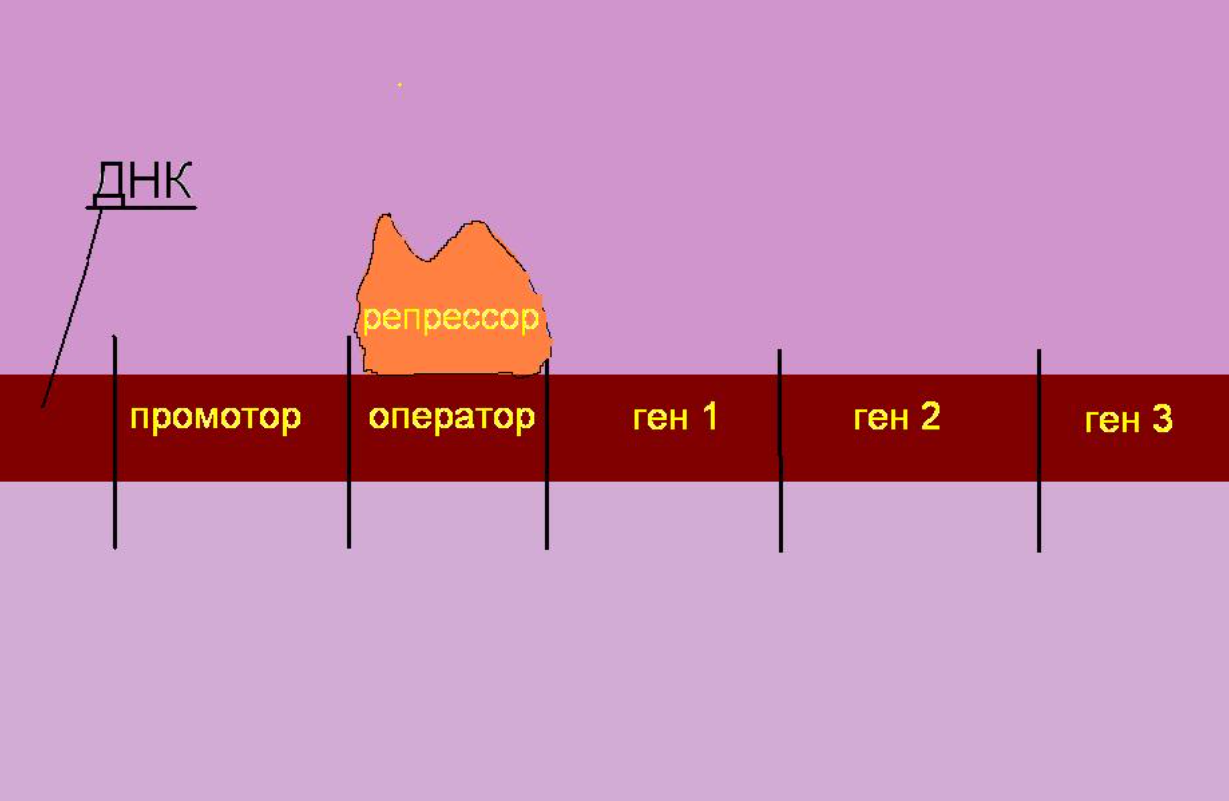
\includegraphics[width = 0.9 \linewidth]{9_glucose_on.png}
        \label{fig:9_glucose_on}
        \caption{Нет лактозы, есть глюкоза. Белок-репрессор подавляет транскрипцию генов поедания лактозы, сидя на операторе (участок оператора так и называется потому, что оперирует транскрипцией).}
    \end{figure}
\end{minipage}
\begin{minipage}{.49\textwidth}
   \begin{figure}[H]
        \centering
        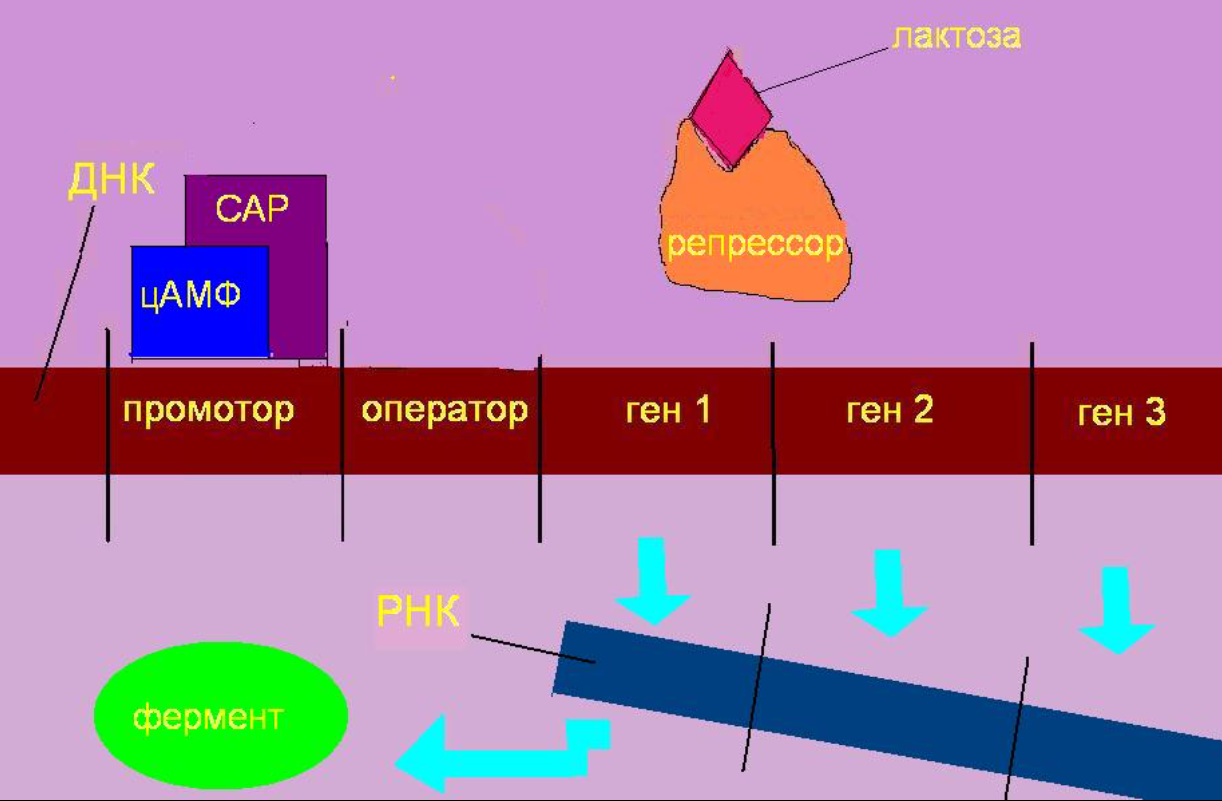
\includegraphics[width = 0.9 \linewidth]{9_lactose_on.png}
        \label{fig:9_lactose_on}
        \caption{Нет глюкозы, есть лактоза. Лактоза связывается с белком-репрессором, белок-репрессор меняет свою форму и больше не держится на ДНК. Приходят белок CAP c цАМФ и упрощают связывание РНК-полимеразы с промотором лактозного оперона.}
    \end{figure}
\end{minipage}

\subsection{Аттенюация на примере 
триптофанового оперона}

\textbf{Триптофановый оперон} — оперон, содержащий гены ферментов, задействованных в биосинтезе аминокислоты триптофан. Далее будем называть его trp-оперон (от англ. tryptophan). 

\textbf{Аттенюация} - способ регулирования транскрипции генов, характерный \textbf{только} для прокариот, у эукариот он не возможен. 

Суть в следующем. У прокариот процессы трансляции и транскрипции происходят одновременно. То есть РНК-полимераза еще не закончила делать РНК по матрице ДНК, а рибосома уже садится на недоделанную РНК и начинает транслировать с нее белки. В случае \textbf{аттенюации} происходит так, что \textbf{процесс трансляции прерывает процесс транскрипции}.

Ниже расписано, как аттенюация происходит на молекулярном уровне в регуляции триптофанового оперона (см. рис. \ref{fig:9_tryptophan}).

\begin{itemize}
    \item В trp-промоторе первая транскрибируемая область называется trpL (от leader), по ней затем рибомосомой транслируется leader peptide (маленький белок).
    
    \item В РНК, построенном по trpL выделяются 4 области - 1, 2, 3 и 4. Они умеют связываться попарно и образовывать петли (см. картинку \ref{fig:9_tryptophan})
    
    \item Важно, что в области 1 есть два последовательно идущих trp-кодона (участки из трех оснований, кодирующие триптофан).
    
    \item За РНК-полимеразой по РНК едет рибосома. Теперь возможно два случая:
    
    а) Пусть сначала в клетке плавает много триптофана. Тогда рибосома, доезжая до области 1, быстро находит два триптофановых аминокислотных остатка и встраивает их в leader peptide. Рибосома проезжает область 1 и закрывает область 2. Области 3 и 4 связываются в петлю. Такая петля вкупе с областью из урацилов не нравится РНК-полимеразе (не знаю почему) и РНК-полимераза тильтует и валит с ДНК, транскрипция прекращается. \textbf{То есть наличие триптофана привело к прекращению собирания синтезирующих его белков}
    
    б) Пусть сначала в клетке плавает мало триптофана. Тогда рибосома, доезжая до области 1, мучительно долго ждет, пока мимо нее проплывет триптофановый аминоксилотный остаток, чтобы встроить его в leader peptide. Области 2 и 3 связываются в петлю, не возникает петли 3-4. РНК-полимеразу ничего не беспокоит и транскриприция доходит до конца, трансляция доходит до конца. \textbf{То есть отсутствие триптофана привело к собиранию синтезирующих его белков}
\end{itemize}

\begin{figure}[H]
    \centering
    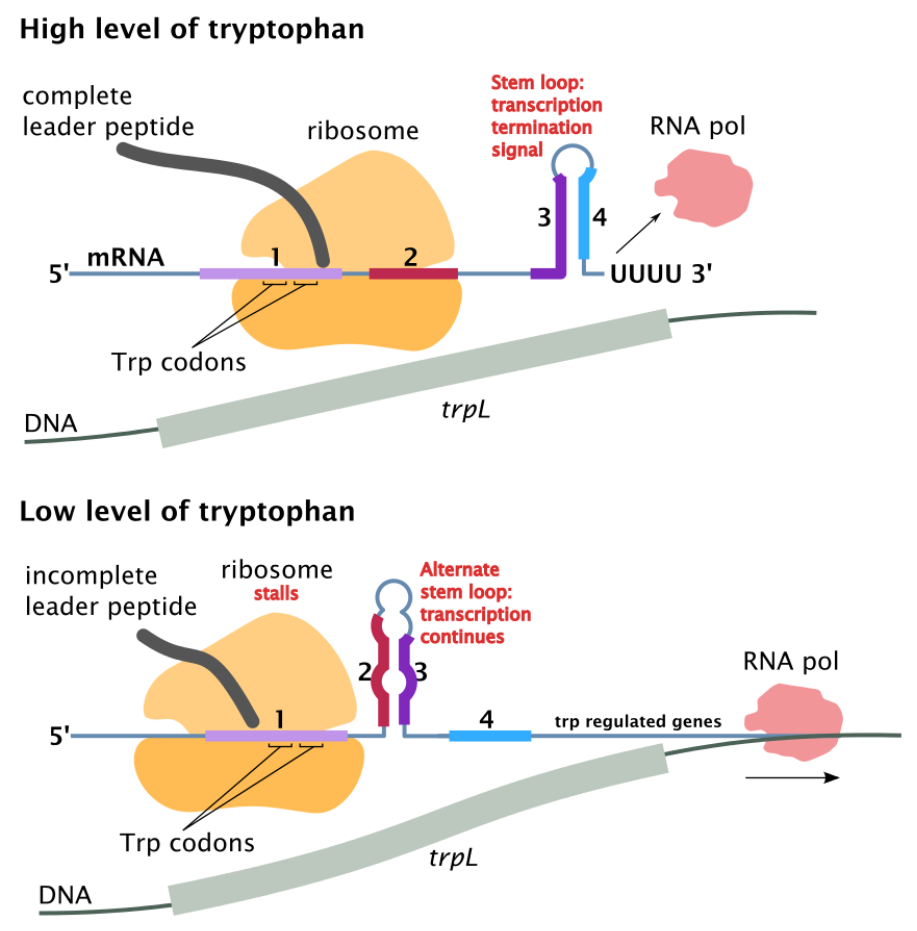
\includegraphics[width = 0.7 \linewidth]{9_tryptophan.png}
    \caption{Аттенюация на примере триптофанового оперона.}
    \label{fig:9_tryptophan}
\end{figure}



\subsection{Промоторы эукариот}

Самое главное отличие эукариотического промотора от прокариотического - \textbf{промотор у каждого гена эукариот свой, оперонов у эукариот нет}.

\subsection{Энхансеры и сайленсеры}
\textbf{Энхансер} (англ. enhancer — усилитель, увеличитель) — небольшой участок ДНК, который после связывания с ним факторов транскрипции стимулирует транскрипцию с основных промоторов гена или группы генов.

\textbf{Сайленсер} - последовательность ДНК, с которой связываются белки-репрессоры транскрипции определенного гена. Связывание белков-репрессоров с сайленсерами приводит к понижению или к полному подавлению синтеза РНК РНК-полимеразой. 

Энхансеры и сайленсеры могут находится на хромосоме (хромосома это комплекс из ДНК и структурных белков гистонов) далеко (даже на другой хромосоме) от промотров генов, транскрипцию которых они регулируют. Тем не менее для их работы необходим физический контакт между ними и промотором. Контакт осуществляется за счёт «выпетливания» ДНК между энхансером/сайленсером и промотором. Молекулярный механизм действия энхансера/сайленсера заключается в том, что он, благодаря собранному на нём белковому комплексу, привлекает/отталкивает РНК-полимеразу II и кофакторы транскрипции в область целевого промотора.

\subsection{Альтернативный сплайсинг}
Между транскрипцией РНК и трансляцией белка у прокариотических клеток ничего не происходит. 

У эукариотических клеток ген состоит из, собственно, участков, кодирующих аминокислоты, составляющие белки, - \textbf{экзонов}, и помойных участков, не кодирующих ничего - \textbf{интронов}. Поэтому после транскрипции гена и до трансляции с него белка у эукариот происходит \textbf{сплайсинг} - вырезание из РНК интронов с оставлением только экзонов.

В результате обычного сплайсинга убираются все интроны, и оставляются все экзоны. А в результате \textbf{альтернативного сплайсинга} получаются самые разные вещи (см. рис. \ref{fig:9_splicing}). Основные вещи, встречающиеся в альтернативном сплайсинге:
\begin{itemize}
    \item пропуск экзона;
    \item удержание интрона (вырезается участок экзона);
    \item взаимоисключающие экзоны (из взаимоисключающих экзонов остается только один);
    \item альтернативный 3'/5' сайт связывания.
\end{itemize}

\begin{figure}[H]
    \centering
    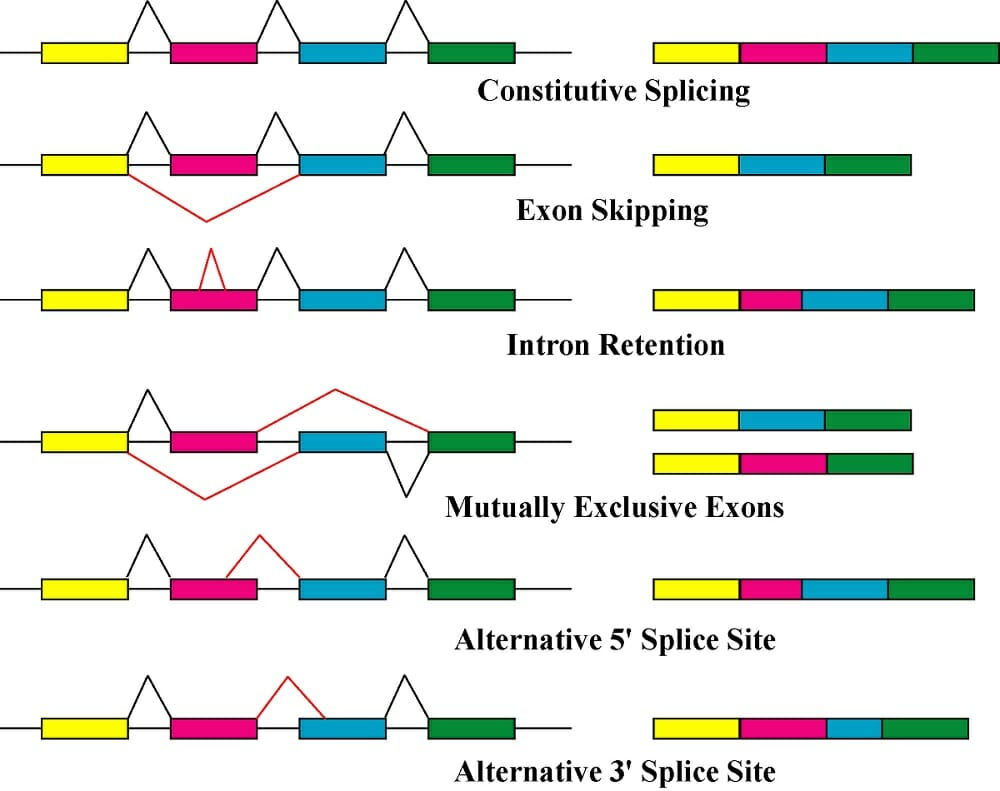
\includegraphics[width = 0.6 \linewidth]{9_splicing.jpg}
    \caption{Вариации альтернативного сплайсинга. В столбце слева мы видим одну и ту же последовательность РНК. Цветные прямоугольники - экзоны, черные линии между ними - интроны. Справа - резьтаты разных процессов альтернативного сплайсинга. В первой строчке обычный сплайсинг.}
    \label{fig:9_splicing}
\end{figure}
